\documentclass[a4paper, 12pt, reqno]{article}
\linespread{1.1}
\usepackage{listings}             % Include the listings-package
\usepackage{xcolor}
\usepackage{graphicx}
\usepackage{float}
\usepackage{amsmath,mathtools,amsthm,amsfonts,amssymb,latexsym,bm}
\usepackage{mathrsfs}
\usepackage{natbib}
\usepackage{textcomp}
\usepackage{gensymb, multicol}
\usepackage{hyperref}
\usepackage{tcolorbox}
\usepackage{caption}
\usepackage{subcaption}
%\usepackage{natbib} 
\usepackage{soul}

\definecolor{codegreen}{rgb}{0,0.6,0}
\definecolor{codegray}{rgb}{0.5,0.5,0.5}
\definecolor{codepurple}{rgb}{0.58,0,0.82}
\definecolor{backcolour}{rgb}{255,255,255}

\lstdefinestyle{mystyle}{
    backgroundcolor=\color{backcolour},   
    commentstyle=\color{codegreen},
    keywordstyle=\color{magenta},
    numberstyle=\tiny\color{codegray},
    stringstyle=\color{codepurple},
    basicstyle=\ttfamily\footnotesize,
    breakatwhitespace=false,         
    breaklines=true,                 
    captionpos=b,                    
    keepspaces=true,                 
    numbers=left,                    
    numbersep=5pt,                  
    showspaces=false,                
    showstringspaces=false,
    showtabs=false,                  
    tabsize=2
}

\lstset{style=mystyle}
\lstset{language=Python}

\renewcommand{\thesection}{}%
\renewcommand{\thesubsection}{}%
\newcommand{\ro}[1]{%
  \xrightarrow{\mathmakebox[\rowidth]{#1}}%
}
\newlength{\rowidth}% row operation width
\AtBeginDocument{\setlength{\rowidth}{3em}}
%\renewcommand\thesubfigure{\arabic{figure}}


\usepackage{blindtext}
\title{EBA3650: Quantitative economics}
\date{\today}
\author{Pauline Malaguti}

\begin{document}

\maketitle
This document was created to gather various explanations for the course Quantitative Economics at BI Norwegian Business School. 
I am not the direct author of the material in this document.
In each part, it is possible to find the original source by clicking on 'Source'. 

\tableofcontents

\newpage
\section{Root Finding}
Root finding refers to the general problem of searching for a solution of an equation $F(x) = 0$  for some function $F$.  
If we want to optimise a function $f(x)$ then we need to find critical points and therefore solve the equation  $f'(x)= 0$. \\
Example quadratic formula: \\
\begin{equation}
x = \frac{-b \pm \sqrt{b^2 - 4ac}}{2a}
\notag
\end{equation}

\href{https://personal.math.ubc.ca/~pwalls/math-python/roots-optimization/root-finding/}{\hl{Source}}

\section{Bisection Method}
The algorithm applies to any continuous function $f(x)$ on an interval a,b where the value of the function $f(x)$ changes sign from $a$ to $b$ . The idea is simple: divide the interval in two, a solution must exist within one subinterval, select the subinterval where the sign of $f(x)$ changes and repeat. \\
\subsection{Algorithm}
The bisection method procedure is:
\begin{enumerate}
  \item Choose a starting interval $[a_0,b_0]$ such that $f(a_0)f(b_0)<0$
  \item Compute $f(m_0)$ where $m_0=(a_0+b_0)/2$ is the midpoint.
  \item Determine the next subinterval $[a_1,b_1]$ :
	\begin{enumerate}
       \item If $f(a_0)f(m_0)<0$, then let $[a_1,b_1]$  be the next interval with $a_1=a_0$ and $b_1=m_0$.
       \item If $f(b_0)f(m_0)<0$, then let $[a_1,b_1]$  be the next interval with $a_1=m_0$ and $b_1=b_0$.
	\end{enumerate}
\item Repeat (2) and (3) until the interval $[a_N,b_N]$ reaches some predetermined length.
\item Return the midpoint value $m_N=(a_N+b_N)/2$
\end{enumerate}
A solution of the equation $f(x)$ on an interval a,b is guaranteed by the \underline{Intermediate Value Theorem} provided $f(x)$ is continuous on $[a,b]$ and \\$f(a)f(b)<0$. In other words, the function changes sign over the interval and therefore must equal 0 at some point in the interval $[a,b]$.
\subsection{Python Implementation}
Write a function called \texttt{bisection} which takes 4 input parameters \texttt{f, a, b} and \texttt{N} and returns the approximation of a solution of $f(x)=0$ given by N iterations of the bisection method. If  $f(a_N)f(b_N)>0$ at any point in the iteration (caused either by a bad initial interval or rounding error in computations), then print "\texttt{Bisection method fails.}" and return \texttt{None}.
\begin{lstlisting}[frame=single]  % Start your code-block
x
def bisection(f,a,b,N):
    '''Approximate solution of f(x)=0 on interval [a,b] by bisection method.

    Parameters
    ----------
    f : function
        The function for which we are trying to approximate a solution f(x)=0.
    a,b : numbers
        The interval in which to search for a solution. The function returns
        None if f(a)*f(b) >= 0 since a solution is not guaranteed.
    N : (positive) integer
        The number of iterations to implement.

    Returns
    -------
    x_N : number
        The midpoint of the Nth interval computed by the bisection method. The
        initial interval [a_0,b_0] is given by [a,b]. If f(m_n) == 0 for some
        midpoint m_n = (a_n + b_n)/2, then the function returns this solution.
        If all signs of values f(a_n), f(b_n) and f(m_n) are the same at any
        iteration, the bisection method fails and return None.

    Examples
    --------
    >>> f = lambda x: x**2 - x - 1
    >>> bisection(f,1,2,25)
    1.618033990263939
    >>> f = lambda x: (2*x - 1)*(x - 3)
    >>> bisection(f,0,1,10)
    0.5
    '''
    if f(a)*f(b) >= 0:
        print("Bisection method fails.")
        return None
    a_n = a
    b_n = b
    for n in range(1,N+1):
        m_n = (a_n + b_n)/2
        f_m_n = f(m_n)
        if f(a_n)*f_m_n < 0:
            a_n = a_n
            b_n = m_n
        elif f(b_n)*f_m_n < 0:
            a_n = m_n
            b_n = b_n
        elif f_m_n == 0:
            print("Found exact solution.")
            return m_n
        else:
            print("Bisection method fails.")
            return None
    return (a_n + b_n)/2


\end{lstlisting}

\href{https://personal.math.ubc.ca/~pwalls/math-python/roots-optimization/bisection/}{\hl{Source}}


\section{Secant method}
The secant method is very similar to the bisection method except instead of dividing each interval by choosing the midpoint the secant method divides each interval by the secant line connecting the endpoints. The secant method always converges to a root of $f(x)$ is continuous on $[a,b]$ and $f(a)f(b)<0$.

\subsection{Secant line formula}
Let $f(x)$ be a continuous function on $[a,b]$ and $f(a)f(b)<0$. A solution of the equation $f(x) = 0$ for $x \in [a,b]$ is guaranteed by the \underline{Intermediate Value} \underline{Theorem}. Consider the line connecting the endpoint values $(a,f(a))$ and $(b,f(b))$. The line connecting these two points is called the secant line and is given by the formula
\begin{equation}
y = \frac{f(b) - f(a)}{b - a}(x - a) + f(a)
\notag
\end{equation}
The point where the secant line crosses the $x$-axis is
\begin{equation}
0 = \frac{f(b) - f(a)}{b - a}(x - a) + f(a)
\notag
\end{equation}
which we solve for $x$
\begin{equation}
x = a - f(a)\frac{b - a}{f(b) - f(a)}
\notag
\end{equation}

\subsection{Algorithm}
The secant method procedure is:
\begin{enumerate}
  \item Choose a starting interval $[a_0,b_0]$ such that $f(a_0)f(b_0)<0$
  \item Compute $f(x_0)$ where $x_0$ is given by the secant line :
\begin{equation}
x_0 = a_0 - f(a_0)\frac{b_0 - a_0}{f(b_0) - f(a_0)}
\notag
\end{equation}
  \item Determine the next subinterval $[a_1,b_1]$ :
	\begin{enumerate}
       \item If $f(a_0)f(m_0)<0$, then let $[a_1,b_1]$  be the next interval with $a_1=a_0$ and $b_1=x_0$.
       \item If $f(b_0)f(m_0)<0$, then let $[a_1,b_1]$  be the next interval with $a_1=x_0$ and $b_1=b_0$.
	\end{enumerate}
\item Repeat (2) and (3) until the interval $[a_N,b_N]$ reaches some predetermined length.
\item Return the value $x_N$, the $x$-intercept of the $N$th subinterval.
\end{enumerate}
A solution of the equation $f(x)$ on an interval a,b is guaranteed by the \underline{Intermediate Value Theorem} provided $f(x)$ is continuous on $[a,b]$ and \\ $f(a)f(b)<0$. In other words, the function changes sign over the interval and therefore must equal 0 at some point in the interval $[a,b]$.

\subsection{Python Implementation}
Write a function called \texttt{secant} which takes 4 input parameters \texttt{f, a, b} and \texttt{N} and returns the approximation of a solution of $f(x)=0$ given by $N$ iterations of the secant method. If $f(a_N)f(b_N)>0$ at any point in the iteration (caused either by a bad initial interval or rounding error in computations), then print "\texttt{Secant method fails.}" and return \texttt{None}.

\begin{lstlisting}[frame=single]  % Start your code-block
x
def secant(f,a,b,N):
    '''Approximate solution of f(x)=0 on interval [a,b] by the secant method.

    Parameters
    ----------
    f : function
        The function for which we are trying to approximate a solution f(x)=0.
    a,b : numbers
        The interval in which to search for a solution. The function returns
        None if f(a)*f(b) >= 0 since a solution is not guaranteed.
    N : (positive) integer
        The number of iterations to implement.

    Returns
    -------
    m_N : number
        The x intercept of the secant line on the the Nth interval
            m_n = a_n - f(a_n)*(b_n - a_n)/(f(b_n) - f(a_n))
        The initial interval [a_0,b_0] is given by [a,b]. If f(m_n) == 0
        for some intercept m_n then the function returns this solution.
        If all signs of values f(a_n), f(b_n) and f(m_n) are the same at any
        iterations, the secant method fails and return None.

    Examples
    --------
    >>> f = lambda x: x**2 - x - 1
    >>> secant(f,1,2,5)
    1.6180257510729614
    '''
    if f(a)*f(b) >= 0:
        print("Secant method fails.")
        return None
    a_n = a
    b_n = b
    for n in range(1,N+1):
        m_n = a_n - f(a_n)*(b_n - a_n)/(f(b_n) - f(a_n))
        f_m_n = f(m_n)
        if f(a_n)*f_m_n < 0:
            a_n = a_n
            b_n = m_n
        elif f(b_n)*f_m_n < 0:
            a_n = m_n
            b_n = b_n
        elif f_m_n == 0:
            print("Found exact solution.")
            return m_n
        else:
            print("Secant method fails.")
            return None
    return a_n - f(a_n)*(b_n - a_n)/(f(b_n) - f(a_n))


\end{lstlisting}
\href{https://personal.math.ubc.ca/~pwalls/math-python/roots-optimization/secant/}{\hl{Source}}

\section{Newton Method}
Newton's method is a root finding method that uses linear approximation. In particular, we guess a solution $x_{0}$ of the equation $f(x)=0$, compute the linear approximation of $f(x)$ at $x_{0}$  and then find the $x$-intercept of the linear approximation.
\subsection{Newton's formula}
Let $f(x)$ be a differentiable function. If  $x_{0}$ is near a solution of $f(x)=0$ then we can approximate $f(x)$ by the tangent line at $x_{0}$ and compute the $x$-intercept of the tangent line. 
The equation of the tangent line at $x_{0}$ is
$$y = f'(x_0)(x - x_0) + f(x_0)$$
The $x$-intercept is the solution $x_{1}$ of the equation
$$0 = f'(x_0)(x_1 - x_0) + f(x_0)$$
and we solve for $x_{1}$
$$ x_1 = x_0 - \frac{f(x_0)}{f'(x_0)} $$
If we implement this procedure repeatedly, then we obtain a sequence given by the recursive formula
$$ x_{n+1} = x_n - \frac{f(x_n)}{f'(x_n)}$$
which (potentially) converges to a solution of the equation $f(x)=0$.

\subsection{Python Implementation}
Write a function called newton which takes 5 input parameters \texttt{f, Df, x0, epsilon} and \texttt{maxinter} 
and returns the approximation of a solution of $f(x)=0$ given by Newton's method. \\
The function may terminate in 3 ways:
\begin{enumerate}
    \item If \texttt{abs(f(xn)) < epsilon}, the algorithm has found an approximate solution and returns \texttt{xn}.
    \item If \texttt{f'(xn) == 0}, the algorithm stops and returns \texttt{None}.
    \item If the number of iterations exceeds \texttt{maxinter}, the algorithm stops and returns \texttt{None}.
\end{enumerate}

\begin{lstlisting}[frame=single]  % Start your code-block
    x
    def newton(f,Df,x0,epsilon,max_iter):
    '''Approximate solution of f(x)=0 by Newton's method.

    Parameters
    ----------
    f : function
        Function for which we are searching for a solution f(x)=0.
    Df : function
        Derivative of f(x).
    x0 : number
        Initial guess for a solution f(x)=0.
    epsilon : number
        Stopping criteria is abs(f(x)) < epsilon.
    max_iter : integer
        Maximum number of iterations of Newton's method.

    Returns
    -------
    xn : number
        Implement Newton's method: compute the linear approximation
        of f(x) at xn and find x intercept by the formula
            x = xn - f(xn)/Df(xn)
        Continue until abs(f(xn)) < epsilon and return xn.
        If Df(xn) == 0, return None. If the number of iterations
        exceeds max_iter, then return None.

    Examples
    --------
    >>> f = lambda x: x**2 - x - 1
    >>> Df = lambda x: 2*x - 1
    >>> newton(f,Df,1,1e-8,10)
    Found solution after 5 iterations.
    1.618033988749989
    '''
    xn = x0
    for n in range(0,max_iter):
        fxn = f(xn)
        if abs(fxn) < epsilon:
            print('Found solution after',n,'iterations.')
            return xn
        Dfxn = Df(xn)
        if Dfxn == 0:
            print('Zero derivative. No solution found.')
            return None
        xn = xn - fxn/Dfxn
    print('Exceeded maximum iterations. No solution found.')
    return None
    
    \end{lstlisting}
\href{https://personal.math.ubc.ca/~pwalls/math-python/roots-optimization/newton/}{\hl{Source}}

Lecture Code: Newton Solver, we try to find $x$ such that $f(x)=0$.
\begin{lstlisting}[frame=single]
# Newton Solver 
def our_newton_solver(funcname,startvalue,arglist):
    ''' Parameters:
            funcname = Function to optmize
            startvalue = Value to start the resesrch of optimal value
            arglist = optimal values for the function
        Returns:
            Optimal value for which the function is solved'''
    current=startvalue
    fval = funcname(current,arglist)
    grad = (funcname(current+0.5*1e-5,arglist)-funcname(current-0.5*1e-5,arglist))*1e+5
    while (abs(fval)>1e-8):
        current = current - fval/grad
        fval = funcname(current,arglist)
        grad = (funcname(current+0.5*1e-5,arglist)-funcname(current-0.5*1e-5,arglist))*1e+5        
    return current 
\end{lstlisting}    

Lecture Code: Newton Maximizer, we try to find $x$ such that $f'(x)=0$.
\begin{lstlisting}[frame=single]
    # Newton Maximizer
def our_newton_maximizer(funcname,startvalue,arglist):
    ''' Parameters:
            funcname = Function to optmize
            startvalue = Value to start the resesrch of optimal value
            arglist = optimal values for the function
        Returns:
            Optimal value for which the function is maximized'''
    current=startvalue
    fval = funcname(current,arglist)
    grad = (funcname(current+0.5*1e-5,arglist)-funcname(current-0.5*1e-5,arglist))*1e+5
    secgrad1 = (funcname(current+0.5*1e-5+0.5*1e-5,arglist)-funcname(current-0.5*1e-5+0.5*1e-5,arglist))*1e+5
    secgrad2 = (funcname(current+0.5*1e-5-0.5*1e-5,arglist)-funcname(current-0.5*1e-5-0.5*1e-5,arglist))*1e+5
    secderiv = (secgrad1-secgrad2)*1e+5
    while (abs(grad)>1e-8):
        current = current - grad/secderiv
        fval = funcname(current,arglist)
        grad = (funcname(current+0.5*1e-5,arglist)-funcname(current-0.5*1e-5,arglist))*1e+5
        secgrad1 = (funcname(current+0.5*1e-5+0.5*1e-5,arglist)-funcname(current-0.5*1e-5+0.5*1e-5,arglist))*1e+5
        secgrad2 = (funcname(current+0.5*1e-5-0.5*1e-5,arglist)-funcname(current-0.5*1e-5-0.5*1e-5,arglist))*1e+5
        secderiv = (secgrad1-secgrad2)*1e+5

    return current 
    \end{lstlisting}  

\section{Utility Functions}
There are several classes of utility functions that are frequently used to generate demand functions. 
\begin{itemize}
    \item One of the most common is the \underline{Cobb-Douglas} utility function, which has the form $$u(x,y) = x^{a}y^{1-a}  \mbox{ with } a \in [0,1]$$
    \item Another common form for utility is the \underline{Constant Elasticity of Substitution (CES)} utility function. This function has the form $$u(x,y) = (ax^{r}+by^{r})^{1/r} $$
    \item A third common utility function is \underline{quadratic}, which has the form  $$u(x,y) = 2ax - (b-y)^{2}$$
\end{itemize}

%\subsection{Cobb-Douglas Utility Function}

\subsection{Constant Elasticity of Substitution (CES)}
The constant elasticity of substitution applied to utility can use the formula
\begin{equation}
    u(x,y) = (ax^{r}+by^{r})^{1/r} \mbox{ where } -\infty <r<1 \mbox{ and } r\neq 0
    \notag
\end{equation}
where r is the subtitution parameter. \\
Marginal rate of substitution (MRS) is computed by
\begin{equation}
    MRS = -\frac{a}{b} \left( \frac{x}{y}\right) ^{r-1}
    \notag
\end{equation}  
The demand functions are computed
\begin{equation}
\begin{split}    
&x(p_x,p_y,I) = \frac{p_{x}^{1/(r-1)}}{p_{x}^{r(r-1)}+p_{y}^{r(r-1)}}\cdot I \\
&y(p_x,p_y,I) = \frac{p_{y}^{1/(r-1)}}{p_{x}^{r(r-1)}+p_{y}^{r(r-1)}}\cdot I
\notag 
\end{split}   
\end{equation} 
where $(p_x,p_y,I)$ are price of good x, price of good y and income. \\
Conquences of variations of $r$:
\begin{itemize}
    \item If $ r \rightarrow 0$ then $u(x,y) \rightarrow$ Cobb Douglas Utility Function $$ u(x,y) = x^{a}y^{1-a}$$
    \item If $ r \rightarrow - \infty $ then $u(x,y) \rightarrow$ Leontief utility Function (inputs are perfect complements) $$ u(x,y) = Min(ay, bx)$$
    \item If $ r \rightarrow 1 $ then $u(x,y) \rightarrow$ Linear Production (inputs are perfect substitutes) $$ u(x,y) = ay + bx$$
\end{itemize} 
\begin{figure}[htp]
    \centering
    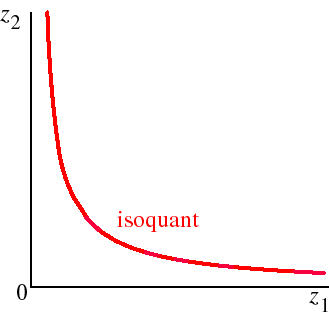
\includegraphics[width=.3\textwidth]{./Curves/CD.png}\hfill
    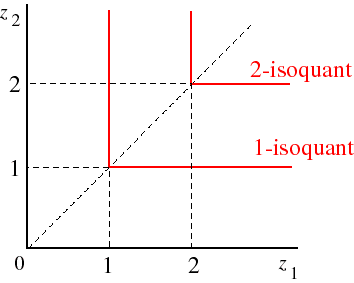
\includegraphics[width=.3\textwidth]{./Curves/C.png}\hfill
    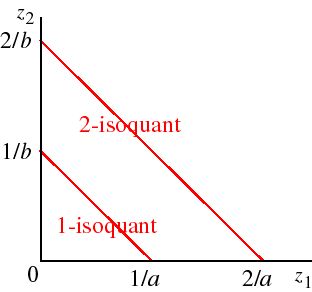
\includegraphics[width=.3\textwidth]{./Curves/S.png}  
    \caption{Utility Curves}
    \label{fig:Utility Curves} 
\end{figure}  

\href{https://en.wikipedia.org/wiki/Constant_elasticity_of_substitution}{\hl{Source}}

\subsection{Quasilinear Utility Functions}
Utility function that is independent of the income effect. 
\begin{equation}
    u(x,y) = v(x) + y
    \notag
\end{equation}
where $v$ is an arbitrary function that is strictly increasing if good $x$ is desired. \\
Indifference curve for $\alpha$ utility level:
\begin{equation}
\begin{split}    
    &v(x) + y = \alpha  \\
    &y = \alpha - v(x)
    \notag 
    \end{split}   
\end{equation} 

Marginal rate of substitution is computed by 
\begin{equation}
    \begin{split}       
    &MRS =\frac{\partial u}{\partial x} / \frac{\partial u}{ \partial y } \\
    &\mbox{where } \frac{\partial u}{\partial x}=v'(x) \mbox{ and } \frac{\partial u}{\partial y} = 1 \\
    &\mbox{Therefore } MRS = v'(x)
    \notag
    \end{split}    
\end{equation}

\href{https://www.core-econ.org/the-economy/book/text/leibniz-05-04-01.html}{\hl{Source}}

\section{Slutsky decomposition: Income and substitution effects}
Slutsky decomposition is the total effect of substitution and income. 

\subsection{Normal Goods}
Normal goods are goods for which demand increases when income increases. 
In the slutsky decomposition, the income and substitution effect reinforce each other when the the good's price change. \\
Income and substitution effects cause an increase in demand when prices decrease. 

\subsection{Income Inferior Goods}
Demand reduced with higher income. \\
Substitution and Income effects oppose each other. When income increases, demand decreases, the substitution effect is the same as normal goods. 

\subsection{Griffon Goods}
Extreme income-inferiority, the income effect may be larger in size than the substitution effect, causing quantity demanded  
demanded to fall as own-prices rises. \\
Slutsky's decomposition of the effect of a price change into a pure substitution effect and an income effect thus explains why the law of downwards-slopping
demand is violated for extremely income-inferior goods.  

\href{https://www.lancaster.ac.uk/staff/desilvad/Varian9e_LecturePPTs_Ch08.pdf}{\hl{Source}}

\section{Microeconomy}
\subsection{The intertemporal utility function}
A plan for consumption in the periods $0, 1, ... , T-1$ is denoted ${c_t}^{T-1}_{t=0}$, where $c_t$ is the consumption in period $t$. We say the plan has \underline{time horizon T}. 
Period 0 (‘the initial period’) need not refer to the ‘birth’ of the household but is just an arbitrary period within the lifetime of the household . \\

We assume that preferences of a household/consumer can be represented by a time-separable intertemporal utility function with a constant utility discount rate and no utility from 
leisure (the latter assumption implies that the labour supply curve of the household in each period is inelastic, ie whatever the changes of prices of labour and leisure the supply of labour stays the same). 
The time-separability itself just means that the intertemporal utility funciton is additive.  \\ 
In addition, we assume geometric utility discounting, meaning that utility obtained $t$ periods ahead is converted into a present equivalent by multiplying by the discount factor $(1 + q)^{-t}$, where $q$ 
is a constant utility discount rate. Hence, $u_t(c_t) = u(c_t)(1 + q)^{-t} $, where $u(c)$ is a time-independent period utility function. Together, these two assumptions amount to
$$ U(c_0, c_1, ..., c_{T-1}) = u(c_0) + \frac{u(c_1)}{(1+q)} + ... +  \frac{u(c_{T -1})}{(1+q)^{T-1}} = \sum_{t = 0}^{T - 1} \frac{u(c_{t})}{(1+q)^{t}} $$

The period utility function is assumed to satisfy $u'(c) > 0 $ and $u''(c) < 0 $.  \\ 
The number $ 1 + q$ tells how many units of utility in the next period the household insists on "in return" for a decrease of one unit of utility in the current period. 
So, a $q > 0$ will reflect that if the chosen level of consumption is the same in two periods, then the individual always appreciates a marginal unit of consumption higher the earlier it arrives. 
This explains why $q$ is named the \underline{rate of time preference} or \underline{rate of impatience}. \\ The utility discount factor, $\frac{1}{1+q}^t$, indicates how many units of utility the household is at most willing to give up 
in period 0 to get one additional unit of utility in period $t$.

Now we assume that the consumer has a utility function over consumption today (time period 0, $t = 0$) and the future (time period 1, $t = 1$). Say, 
$$ u(c_{t = 0},c_{t = 1}) = c_{t = 0}^{\alpha} + \frac{1}{1+q} * c_{t = 1}^{\alpha} $$ 
where $\alpha$ is a parameter between 0 and 1, say 0.5, and $q$ is a given number for instance 0.04. 
The consumer has some income/endowment ($e$ or $I$)in both periods but can also save or borrow money. Savings $s$ is given by 
$$ s = e_0 - c_{t = 0} $$ 
and consumption in period 2 is given by 
$$ c_{t = 1} = e_1 + s \times (1+r)$$ 
where $r$ is the interest rate ($s$ will be negative if the consumer borrows money.) Since $e_1$ is in tomorrow's money, we have to multiply the savings we bring forward by $(1 + r)$ to We can put this into our 
numerical framework by substituting for $s$, giving a budget constraint 
$$ c_{t = 1} = e_1+ (e_0- c_{t = 0}) \times (1+r)$$
\href{https://web.econ.ku.dk/okocg/VM/VM-general/Kapitler%20til%20bog/Ch9-2016-1.pdf}{\hl{Source}} \\

Code: Visualise the changes in consumption combination (indifference curve) when the interest rate varies. 
\begin{lstlisting}[frame=single]
def f(rs,arglist):
    e = arglist[0] ; q = arglist[1]
    for element in range(len(rs)):
    r = rs[element]

    def utility(c1, c2):
        #e = 0.5 ; q = 0.04
        return np.power(c1,e)+(1/(1+q))*np.power(c2,e)

    def utility_budget(c1, ip_list):
        I1 = ip_list[0] ; I2 = ip_list[1] ; r = ip_list[2]
        c2 = I2 + (I1 - c1)*(1+r)
        return utility(c1, c2)
        
    def demand(I1, I2, r):
        c1 = newton_max(utility_budget, 0.1, [I1, I2, r])
        c2 = I2 + (I1 - c1)*(1+r)
        return c1, c2

    def indiff_dist(c2, mylist): 
        c1 = mylist[0] ; utility_level = mylist[1]
        utitility_achieved = utility(c1,c2)
        return utitility_achieved - utility_level

    def indifference(c1, util):
        return newton_add(indiff_dist, 1, [c1,util])

    def indirect_utility(I1, I2, r):
        c11, c22 = demand(I1, I2, r)
        return utility(c11, c22)

    # initialise quantiites of good 1 (x), income (I), and prices of the two goods
    c1 = np.linspace(1,30,100) ; I1 = 10 ; I2 = 12

    # get indirect utility curve here
    utility_level = indirect_utility(I1, I2, r)
    c2 = np.zeros(len(c1))

    for idx in range(len(c1)):
        c2[idx] = indifference(c1[idx], utility_level)


    #Compute the optimal demand for each r
    dem = []
    dem= demand(I1,I2,r)    

    # plot and make nice
    plt.figure(figsize = (6,4)) ; plt.plot(c1, c2, label = f'Indifference curve with r = {np.round(r,2)}')
    plt.plot(c1, I2 + (I1 - c1)*(1+r), color = 'red', label = 'budget line')
    plt.scatter(dem[0],dem[1], label = "Optimum demand", color ='black')
    plt.text(dem[0], dem[1], '({}, {})'.format(np.round(dem[0],2), np.round(dem[1],2)))
    plt.xlabel('quantity of goods consumed today') ; plt.ylabel('quantity of good s consumed tomorow')
    plt.legend(loc = 'upper right')
    plt.title('Evolution of indifference curves when interest rates varie')
    plt.xlim(0,30) ; plt.ylim(0,30)
    plt.show()

\end{lstlisting} 
\hfill
Code: Visualise Slutsky decomposition to determine consumer's behaviour. 
\begin{lstlisting}[frame=single]
    def utility(c1, c2):
    e = 0.5 ; q = 0.04
    return np.power(c1,e)+(1/(1+q))*np.power(c2,e)

def utility_budget(c1, ip_list):
    I1 = ip_list[0] ; I2 = ip_list[1] ; r = ip_list[2]
    c2 = I2 + (I1 - c1)*(1+r)
    return utility(c1, c2)
    
def demand(I1, I2, r):
    c1 = newton_max(utility_budget, 0.1, [I1, I2, r])
    c2 = I2 + (I1 - c1)*(1+r)
    return c1, c2

def indiff_dist(c2, mylist): 
    c1 = mylist[0] ; utility_level = mylist[1]
    utitility_achieved = utility(c1,c2)
    return utitility_achieved - utility_level

def indifference(c1, util):
    return newton_add(indiff_dist, 1, [c1,util])

def indirect_utility(I1, I2, r):
    c11, c22 = demand(I1, I2, r)
    return utility(c11, c22)

def diff_indirect_utilities(income_to_be_found,longlist):
    I1 = longlist[0] ; I2 = longlist[1] ; r1 = longlist[2] ; r2 = longlist[3]
    return indirect_utility(I1, I2, r1) - indirect_utility(I1,income_to_be_found,r2)

# define the parameters
I1 = 12 ; I2 = 8 ; r1 = 0.1 ; r2 = 0.85


# Give optimal income level for period 2 when prices change
a = newton_add(diff_indirect_utilities, 1, [I1, I2, r1, r2])
# print(a)

c1 = np.linspace(0.1, 10, 100) # quantity of good today

# plot with the new budget line as well
plt.figure(figsize = (12, 8))

# budget curve 1 : Before changes
plt.plot(c1, I2 + (I1 - c1)*(1+r1), color = 'pink', label = 'budget curve 1')

# budget curve2 : After changes
plt.plot(c1, a + (I1 - c1)*(1+r2), color = 'red', label = 'budget curve with a')

# get the utility levels
u_bar = indirect_utility(I1, I2, r1) 
u_bar2 = indirect_utility(I1, I2, r2)

#print(u_bar, u_bar2)

# express utility max as a function of quantity of good tomorrow
c21 = np.zeros((100,1)) ; c22 = np.zeros((100,1))

for idx in range(len(c1)):
    c21[idx] = indifference(c1[idx], u_bar)
    c22[idx] = indifference(c1[idx], u_bar2)

plt.plot(c1, c21, label = 'indifference curve 1', color = 'green') 
plt.plot(c1, c22, label = 'indifference curve 2', color = 'blue')

# find utility-maximising consumption bundle
dems1 = demand(I1, I2, r1) ; plt.scatter(dems1[0], dems1[1],s=50,alpha=0.5,color='black')
dems2 = demand(I1, I2, r2) ; plt.scatter(dems2[0], dems2[1],s=50,alpha=0.5,color='black')

# make nice
# plt.vlines(dems1[0], 8, 10.5, linestyles = 'dotted', color = 'k')
# plt.vlines(dems2[0], 8, 10.5, linestyles = 'dotted', color = 'k')
plt.annotate('A', xy = (dems1[0], dems1[1]), xycoords='data',rotation = 30, size=15)
plt.annotate('B', xy = (dems2[0], dems2[1]), xycoords='data',rotation = 30, size=15)

plt.vlines(dems1[0],0,dems1[1],linestyles='dotted')
plt.vlines(dems2[0],0,dems2[1],linestyles='dotted')
plt.hlines(dems1[1],0,dems1[0], linestyles='dotted')
plt.hlines(dems2[1],0,dems2[0], linestyles='dotted')
plt.ylim(0,40) ; plt.xlim(0,10)
plt.title('Income and Substitution effect: Consequences on consumption in time')
plt.xlabel('consumption today, c1') ; plt.ylabel('consumption tomorrow, c2')
plt.legend(loc = 'upper right') 

\end{lstlisting}
Then to determine the consumer's behaviour you compute the savings for the first period (today). 
\begin{lstlisting}[frame=single]
s = I1 - dems1[0]
# where dems1[0] is the consumer of today's goods
\end{lstlisting}  
If the savings are negative then the consumer is a borrower, if savings are positive then the consumer is a saver. 
To visualise both cases you can play with the values of Incomes (I1 and I2) and the rates (r1 and r2).  

\subsection{Monopoly}
A monopoly consists of one firm that produces a unique product or service with no close substitutes. Entry into the market is blocked, which gives the firm market power (i.e., the power to raise price above marginal cost).\\
Some definitions,
\begin{itemize}
\item Average revenue = market demand curve. 
\item Marginal revenue: change in revenue resulting from a one-unit increase in output. 
    \begin{itemize}
        \item $MR > 0 \mbox{} \rightarrow$ Revenue increases
        \item $MR < 0 \mbox{} \rightarrow$ Revenue decreases
        \item When the demand curve is downward sloping, the price ($=AR$) is above MR for all units sold at the same price.
        \item No supply curve in monopolistic markets. That is, there is a one-to-one relationship between price and the quantity produced

    \end{itemize}
\end{itemize}
\underline{Profit Maximization for Monopolists} \\
All profit maximizing firms, regardless of the structure of the markets in which they sell, maximize profits by setting output such that marginal revenue equals marginal cost. \\
Monopolists are ‘price makers’ in the sense that they can set their prices by picking a point on the demand curve. Note that they are not free of constraint; the demand curve dictates the maximum price they can charge for every quantity level. The task for the profit-maximizing monopolist is to determine which point on the demand curve maximizes their profits. A downward sloping demand curve will mean that the firm faces a trade-off: they can sell more but must lower their price to do so. This means that the marginal revenue of a monopolist will depend on their output decision. \\

The total revenue for a firm is the amount of goods they sell, $Q$, multiplied by the price at which they sell the goods, $p$. Note that $Q$ is both the firm’s output and the market output as there is only the one firm supplying the market. 
$$ TR = p\times Q$$
The firm’s marginal revenue is the change in total revenue from the sale of one more unit of their output. Thus a firm that earns $\Delta TR$ extra revenue from the sale of $\Delta Q$ more units has a marginal revenue of: 
$$MR = \frac{\partial TR}{\partial Q}$$
Dividing both sides by ∆Q gives us an expression for marginal revenue:
$$MR= p+Q\frac{\Delta p}{\Delta Q}$$
The first part, $p$, is the extra revenue the firm gets from selling an extra unit of the good. The second part, $Q\frac{\Delta p}{\Delta Q}$ , which is negative, is the decrease in revenue from the fact that increasing output marginally, 
lowers the price the firm receives for all of its output. Since the second part is negative we know that the MR curve is below the demand curve for every Q since demand curve relates price and quantity. \\

A profit maximizing firm chooses output such that the marginal cost of producing that output exactly matches the marginal revenue it gets from selling that output. The intersection of the marginal revenue and marginal cost curves occurs at point $Q^M $ and the highest price at which the monopolist can sell exactly $Q^M $ is $p^M $. 
At $Q^M $ the total revenue is simply $(p^M ) \times (Q^M )$, and total cost is $(AC) \times (Q^M )$ since AC is just $\frac{TC}{Q}$. \\

Suppose the demand for a good produced by a monopolist is $p = A - BQ$. Note that this is an \underline{inverse demand curve} a demand curve written with price as a function of quantity. We can find the marginal revenue curve by first noting that $TR = p \times Q$. 
Thus $TR = (A - BQ) \times Q$, or $TR = AQ - BQ^{2}$. 
In other words, for an inverse demand curve, $p = A - BQ$, the marginal revenue curve is $MR = A - 2BQ$. \\

\href{https://open.oregonstate.education/intermediatemicroeconomics/chapter/module-15/}{\hl{Source}}

\subsection{Expenditure functions}
The expenditure function gives the \underline{minimum amount of money} an individual needs to spend to achieve some level of utility, given a utility function and the prices of the available goods. \\
Say the utility we want to achieve is $\alpha$ for $n$ number of comodities at a price vector $p$. The expenditure function is then:
$$ e(p, \alpha) = \underset{x \in \geq (\alpha)}{min} p \cdot x$$
where $ x \in \geq \alpha$ means that we have consumption bundles that give at least the same utility level as $\alpha$. \\
Properties of the expenditure function :
\begin{itemize}
    \item The function is continuous in $p$ and $u$ 
    \item The function is nondecreasing in $p$ and strictly increasing in $u$ provided $p \gg 0$ 
    \item The function is concave in $p$
    \item If the utility function is quasi-concave, the \hyperlink{thesentence}{Shephard's Lemma} can be applied to the expenditure function. 
\end{itemize}

\begin{tcolorbox}
    \hypertarget{thesentence}{Shephard's Lemma} \\
    The lemma states that if the indifference curves of the expenditure or cost function are convex, then the cost minimizing point of a given good $i$ with price $p_i$ is unique. \\ The idea is that a consumer will 
    buy a unique ideal amount of each item to minimize the price for obtaining a certain level of utility given the price of goods in the market. \href{https://en.wikipedia.org/wiki/Shephard%27s_lemma}{(Source)}
\end{tcolorbox}
    
\href{https://en.wikipedia.org/wiki/Expenditure_function}{\hl{Source}}

\subsection{Hicksian demand function}
A consumer's Hicksian demand function or compensated demand function for a good is his quantity demanded as part of the solution to minimizing his expenditure on all goods while delivering a fixed level of utility. \\ Essentially, a Hicksian demand function shows how an 
economic agent would react to the change in the 
price of a good, if the agent's income was compensated to guarantee the agent the same utility previous to the change in the price of the good—the agent will remain on the same indifference curve before and after the change in the price of the good.

The demand curve we usually refer to is the Marshallian demand function. The Marshallian demand function and the Hicksian demand function are related :
$$h(p,u) = x(p,e(p,u)),$$
where $e(p,u)$ is the expenditure function ; and by:
$$h(p, v(p,w)) = x(p,w),$$
where $v(p,w)$ is the indirect utility function (which gives the utility level of having a given wealth under a fixed price regime). \\
The two demand functions are still difference in the sense that Marshallian demand comes from the Utility Maximization Problem, while the Hicksian Demand comes from the Expenditure Minimization Problem.

\underline{Compensation of prices changes} \\
The Hicksian demand function isolates the substitution effect by supposing the consumer is compensated with exactly enough extra income after the price rise to purchase some bundle on the same indifference curve. If the Hicksian demand function is steeper than the Marshallian demand, the good is a normal good; otherwise, the good is inferior. 
Hicksian demand always slopes down.
\begin{tcolorbox}
    Marshallian demand function\\
    Marshallian demand curves show the effect of price changes on quantity demanded. As the price of a good rises, ordinarily, the quantity of that good demanded will fall, but not in every case. 
    The price rise has both a substitution effect and an income effect. The substitution effect is the change in quantity demanded due to a price change that alters the slope of the budget constraint but leaves the consumer on the same indifference curve 
    (i.e., at the same level of utility). The substitution effect always is to buy less of that good. The income effect is the change in quantity demanded due to the effect of the price change on the consumer's total buying power. 
\end{tcolorbox}
\href{https://en.wikipedia.org/wiki/Hicksian_demand_function}{\hl{Source}}

\subsection{Walras's law}
Walras's law is a principle in general equilibrium theory asserting that budget constraints imply that the values of excess demand (or, conversely, excess market supplies) 
must sum to zero regardless of whether the prices are general equilibrium prices. \\
\underline{Premilaries definitions}
\begin{itemize}
    \item A market for a particular commodity is in equilibrium if, at the current prices of all commodities, the quantity of the commodity demanded by potential buyers equals the quantity supplied by potential sellers.
    \item An economy is in general equilibrium if every market in the economy is in partial equilibrium.
    \item 'Excess demand' refers to a situation in which a market is not in equilibrium at a specific price because the number of units of an item demanded exceeds the quantity of that item supplied at that specific price. 
    Excess demand yields an economic shortage. A negative excess demand is synonymous with an excess supply, in which case there will be an economic surplus of the good or resource. 'Excess demand' may be used more generally to refer to the 
    algebraic value of quantity demanded minus quantity supplied, whether positive or negative.
\end{itemize}
\underline{Formal Statement} \\
For every agent $i$, let $E_i$ be their initial endowment vector and $x_i$ their Marshallian demand function. 
Given a price vector $p$, the income of the consumer $i$ is $p \cdot E_i$. Hence their demand vector is $x_i(p,p\cdot E_i)$.  \\
The excess in demand function is computed by: $$ z(p) = \sum_{i=1}^{n} (x_i(p \cdot E_i) - E_i) $$
The budget constraint here is : $$p \cdot x_i = p \cdot E_i \mbox{ for each } i$$
The excess in demand can be rewritten as $$ p \cdot z(p) = \sum_{i=1}^{n} (p \cdot x_i(p \cdot E_i) -  p \cdot E_i) $$
which can be simplified as $$p \cdot z(p) = 0$$
\href{https://en.wikipedia.org/wiki/Walras%27s_law}{\hl{Source}}

\subsection{Edgeworth box}
In economics, an Edgeworth box (or Edgeworth-Bowley box), is a graphical representation of a closed market with just two commodities, X and Y, and two consumers. 
The dimensions of the box are the total quantities $\Omega_x$ and $\Omega_y$ of the two goods. \\
Let the consumers be Octavio and Abby. The top right-hand corner of the box represents the allocation in which Octavio holds all the goods, while the bottom left corresponds to complete ownership by Abby. 
Points within the box represent ways of allocating the goods between the two consumers.
Market behaviour will be determined by the consumers' indifference curves. The blue curves in the diagram represent indifference curves for Octavio, and are shown as convex from his viewpoint (i.e. seen from the bottom left). 
The orange curves apply to Abby, and are convex as seen from the top right. Moving up and to the right increases Octavio's allocation and puts 
him onto a more desirable indifference curve while placing Abby onto a less desirable one. 
\begin{figure}[H]
    \centering
    \includegraphics[width=.38\textwidth]{./Curves/Edgeworthexample1.png}
    \caption{An Edgeworth box}
    \label{fig: An Edgeworth box} 
\end{figure}  
Convex indifference curves are considered to be the usual case. 
They correspond to diminishing returns for each good relative to the other.
Exchange within the market starts from an initial allocation known as an endowment. \\

\underline{Market Equilibrium} \\
Since there are only two commodities the effective price is the exchange rate between them. Our aim is to find the price at which market equilibrium can be attained, which will be a point at which no further 
transactions are desired, starting from a given endowment. These quantities will be determined by the indifference curves of the two consumers.
We shall assume that every day Octavio and Abby go to market with endowments $(\omega_x, \omega_y )$ and $(\Omega_x - \omega_x , \Omega_y - \omega_y )$ of the two commodities, corresponding to the position $\mathbf{\omega}$. 
in the diagram. The two consumers will exchange between themselves under competitive market behaviour. \\
If two X's exchange for a single Y, then Octavio's and Abby's transaction will take them to some point along the solid grey line, which is known as a budget line.
Budget lines for a couple of other prices are also shown as dashed and dotted lines in Fig. 3.a.
The equilibrium corresponding to a given endowment $\omega$ is determined by the pair of indifference curves which have a common tangent such that this tangent passes through $\omega$. We will use the term 'price line' to denote a common tangent to two indifference curves. 
An equilibrium therefore corresponds to a budget line which is also a price line, and the price at equlibrium is the gradient of the line. 
In Fig.3.b.  $\omega$ is the endowment and $\omega '$ is the equilibrium allocation.
\begin{figure}[H]
    \centering
    \begin{subfigure}{0.4\textwidth}
        \includegraphics[width=\textwidth]{./Curves/Edgeworthexample2.png}
        \caption{Edgeworth box market}
        \label{fig:3a}
    \end{subfigure}
    \hfill
    \begin{subfigure}{0.4\textwidth}
        \includegraphics[width=\textwidth]{./Curves/Edgeworthexample3.png}
        \caption{Equilibrium in an Edgeworth box}
        \label{fig:3b}
    \end{subfigure}
    \hfill
    \begin{subfigure}{0.4\textwidth}
        \includegraphics[width=\textwidth]{./Curves/Edgeworthexample4.png}
        \caption{Division of a neighbourhood by crossing indifference curves}
        \label{fig:3c}
    \end{subfigure}
            
    \caption{Edgeworth boxes}
    \label{fig:two curves}
\end{figure}

Firstly, any point in the box must lie on exactly one of Abby's indifference curves and on exactly one of Octavio's. If the curves cross (as shown in Fig. 3.c.) then they divide the immediate neighbourhood into four regions, 
one of which (shown as pale green) is preferable for both consumers; therefore a point at which indifference curves cross cannot be an equlibrium, and an equilibrium must be a point of tangency.
Secondly, the only price which can hold in the market at the point of tangency is the one given by the gradient of the tangent, since at only this price will the consumers be willing to accept limitingly small exchanges.
And thirdly (the most difficult point) all exchanges taking the consumers on the path from $\omega$ to equilibrium must take place at the same price. 
If this is accepted, then that price must be the one operative at the point of tangency, and the result follows. \\

\underline{Pareto Set} \\
An allocation of goods is said to 'Pareto dominate' another if it is preferable for one consumer and no worse for the other. An allocation is said to be 'Pareto optimal' (or 'Pareto efficient') if no other allocation Pareto dominates it. The set of Pareto optimal allocations is known as the Pareto 
set (or 'efficient locus'). \\
Consider a pair of tangential curves, one for each consumer as illustrated in Fig. 4.a., where the point of tangency is shown by the purple dot. Then convexity guarantees that the curves cannot intercept other than at the point of tangency, and the box is accordingly divided into 3 regions. The pale blue 
area is preferable to the point of tangency for Octavio but worse for Abby; the pale orange area is preferable for Abby but worse for Octavio; and the white area is worse for both. Similar 
considerations apply to the boundaries. It follows that the point of tangency is Pareto optimal. \\ 
Thus the Pareto set is the locus of points of tangency of the curves. This is a line connecting Octavio's origin (O) to Abby's (A). An example is shown in Fig. 4.b., where the purple line is the Pareto set corresponding to the indifference curves for the two consumers.
\begin{figure}[H]
    \centering
    \begin{subfigure}{0.4\textwidth}
        \includegraphics[width=\textwidth]{./Curves/pareto1.png}
        \caption{Division of the box by two tangential indifference curves}
        \label{fig:4a}
    \end{subfigure}
    \hfill
    \begin{subfigure}{0.4\textwidth}
        \includegraphics[width=\textwidth]{./Curves/pareto2.png}
        \caption{Pareto set (purple line) for an Edgeworth box}
        \label{fig:4b}
    \end{subfigure}
            
    \caption{Pareto Set}
    \label{fig:pareto curves}
\end{figure}

\href{https://en.wikipedia.org/wiki/Edgeworth_box}{\hl{Source}}

%\bibliography{myrefs, hisrefs, herrefs}

%\bibliographystyle{apalike} 
%\nocite{*}
%\bibliography{myrefs}

\end{document}

